\chapter{Architectural Design}
\section{Overview: high-level components and interactions}

As anticipated in the previous chapter, the architecture selected for the design and development of the system is the three-tier architecture.

This architecture allow us to split the implementation into three layers:
\begin{enumerate}
	\item Presentation: it is the online web page that will be used by the CPOs to access all the information and settings of their charging stations
	\item Application: is the backend of the system, dove sono implementati all the logics related to the energy management by the stations, the management of reservations, the interactions with the various eMPS and the DSOs.
	\item Data: is the layer responsible to expose connectivity interfaces from the database. It will be a DBMS.
\end{enumerate}

All the layers communicate in a linear way: the Presentation one interacts only with the Application layer, the same as the Data layer. With this architecture the presentation and the Data layers have no direct communication path.
Other advantages of using this architecture are that the various layers can be developed with different technologies and that they can be duplicated and differentiated.

The main reasons behind the choice are:
\begin{itemize}
	\item We are not the producer of the data
	\item We need to integrate different external services
	\end{itemize}
\end{itemize}


\begin{figure}[h]
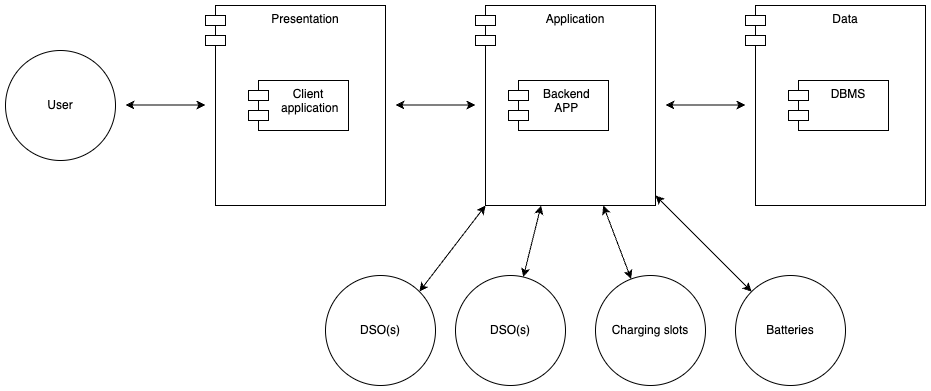
\includegraphics[width=\textwidth]{component_diagrams/overview}
\caption{Overview of the chosen three-tier architecture with actors}
\end{figure}

\clearpage

\section{Component view}
The following schema shows all the main components and interfaces of the system. Later on you will find the details of each component.


\begin{figure}[h]
\centering
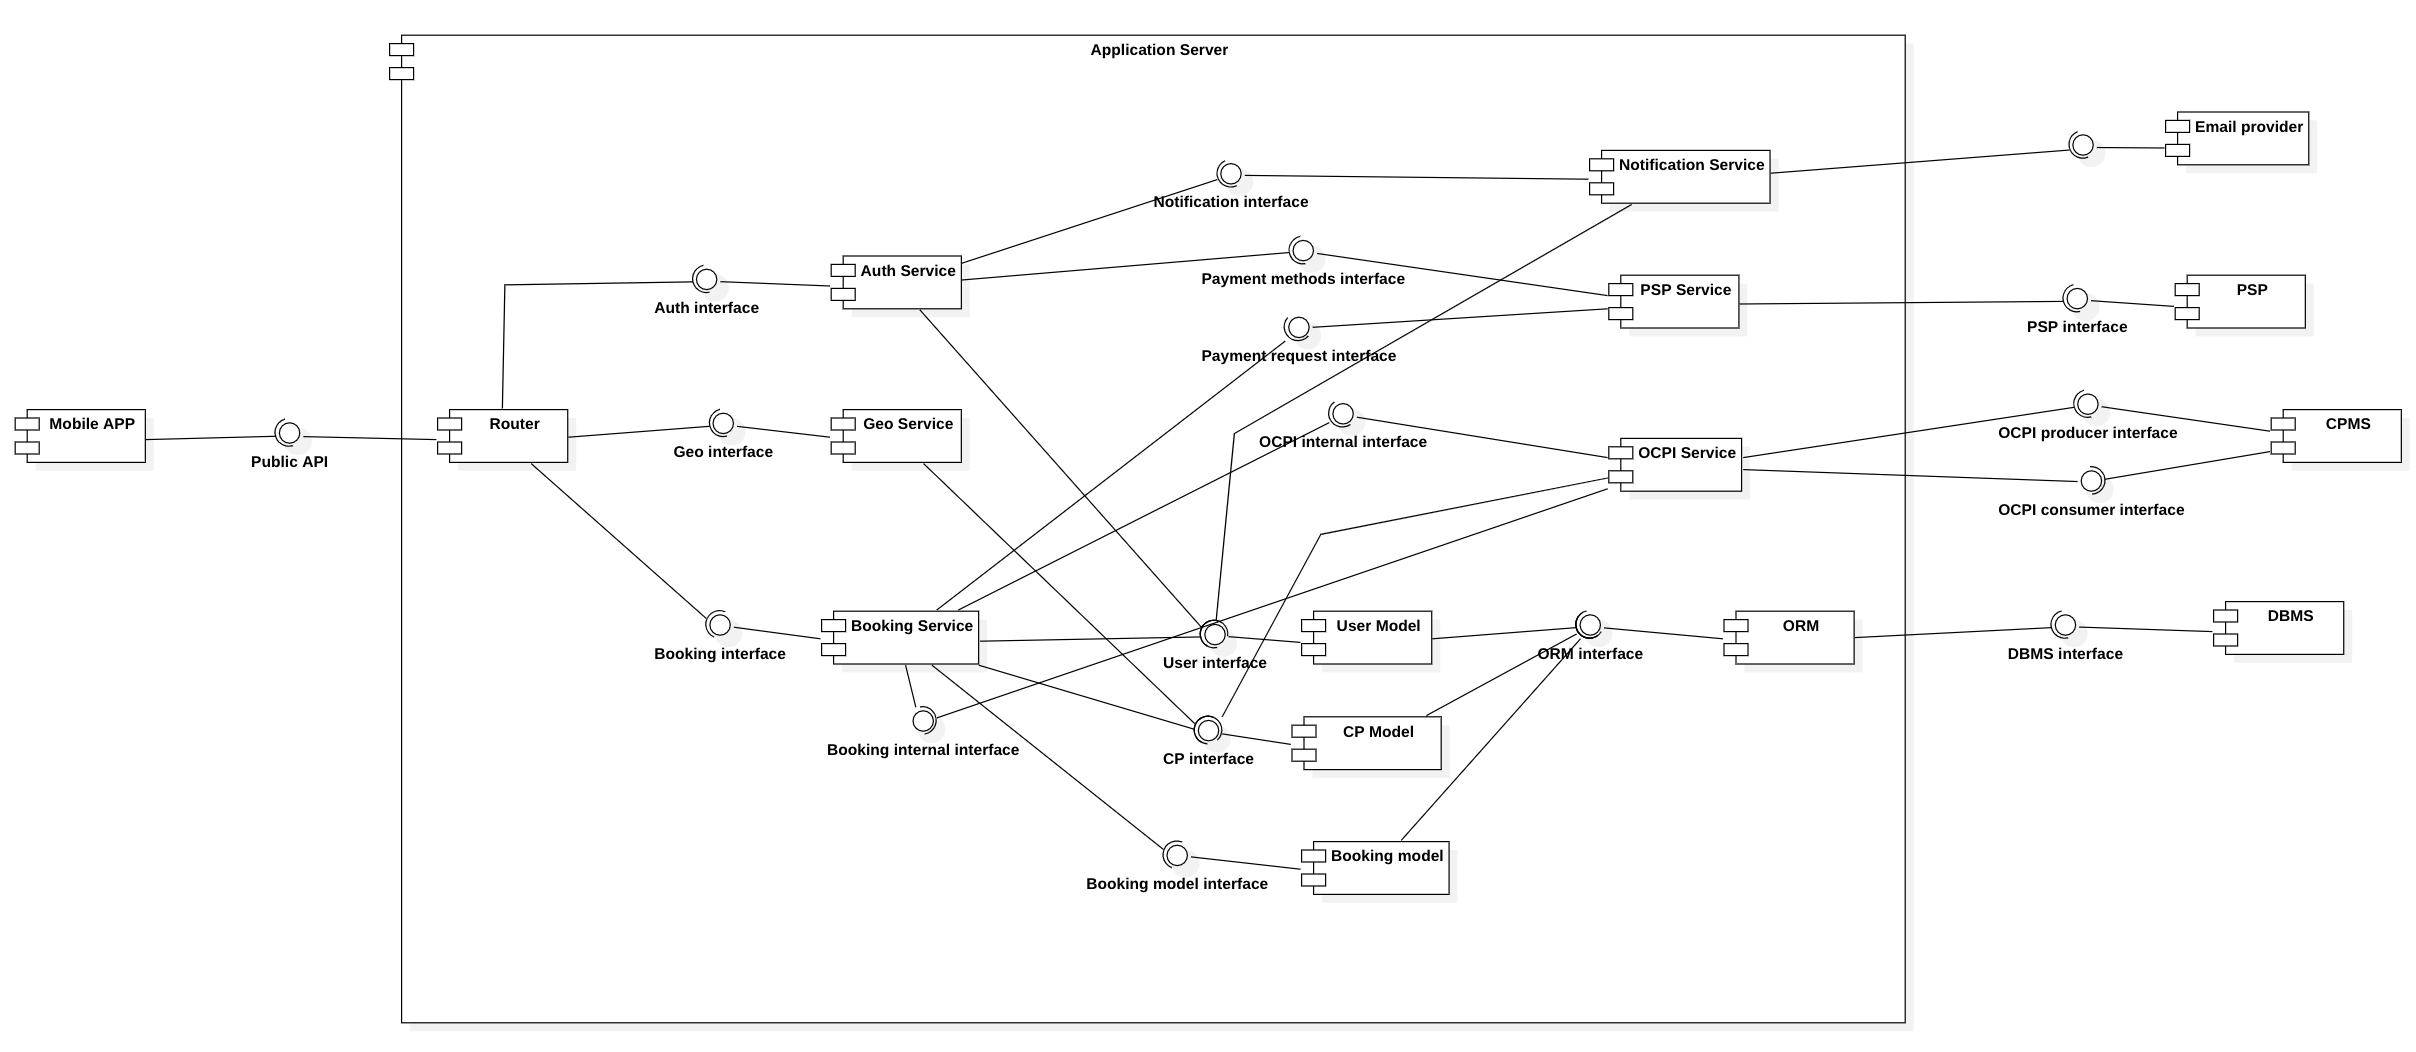
\includegraphics[angle=90,origin=c,height=14cm]{component_diagrams/component_diagram}
\caption{Component diagram of the system}
\end{figure}

\clearpage
\newpage

\begin{itemize}
	\item \textbf{Application server}: not a real "component" it shows the division between the backend, the frontend, the data layer and the external service. In the three-tier architecture it represents the Application layer.
	\item \textbf{eMSP}: e-Mobility Service Provider that exposes OCPI compliant API
	\item \textbf{ClienApplication}: web application for the system, used by the users.
	\item \textbf{External Status Service}: Service that provides information regarding the external status of the charging station. informations like number of charging sockets available, their type such as slow/fast/rapid, their cost, and, if all sockets of a certain type are occupied, the estimated amount of time until the first socket of that type is freed.
	\item \textbf{Internal Status Service}:Service that provides information regarding the internal status like: the amount of energy stored in the batteries, if any, the quantity of vehicles currently being charged, and the current energymanagement settings.
	\item \textbf{Dynamic pricing Service}:Service that manages and imposes the tariff for each type of charge and period, taking into consideration the current energy price and the current energy management settings. A tariff can also be set using a special function.
	\item \textbf{Energy Management Service}: Component that dynamically decides which DSOs to draw energy from, controlling the use of the batteries present at the charging stations
	\item \textbf{DSO Service}: it manages the communication with the Distribution System Operators DSO
	\item \textbf{OCPP Service}: it manages the communication with the Charge slot (EVSE)
	\item \textbf{Carge slot}: Physical device with multiple Connectors that can charge electric vehicles
	\item \textbf{Battery}: Battery physically present at some charging stations
	\item \textbf{Router}: handles all the requests directed to the Application APIs that comes into the Application Server, uses the Auth Service to Authenticate and Authorize them. After that, if all the checks are passed, it will forward the request to the correct service that exposes the required route. It basically acts as a middleware, its presence is useful as it acts as a single point to develop all the authentication/authorization logic so that if it needs changes we can just update the router (and eventually the auth service) instead of updating all the services.
	\item \textbf{Auth Service}: is an internal service that handles authentication (Signup and login) and authorization (even if at the moment our system does not need that).
	\item \textbf{Booking Service}: it manages the booking for the application, it exposes some endpoints to the router for the booking functionalities of the eMSP it also manages charging sessions.
	\item \textbf{OCPI Service}: it manages the communication with the eMSP, it exposes the endpoints for the PUSH part of the protocol (is needed to send real-time updated to eMSP )
	\item \textbf{ORM}: a library that allows an easy to use mapping between Models and DB table, it handles queries and relationships. It is not worth it to develop an in-house solution, so we will use a library for that.
	\item \textbf{User Model, CP Model, Booking Model, Tariff Model, System settings Model }: Models components that sit between services and ORM, useful to attach event listeners and other effects that need to run when updating the data. 
	\item \textbf{DBMS}: Database Management System
\end{itemize}

\subsection{Class diagram}
\begin{figure}[h]
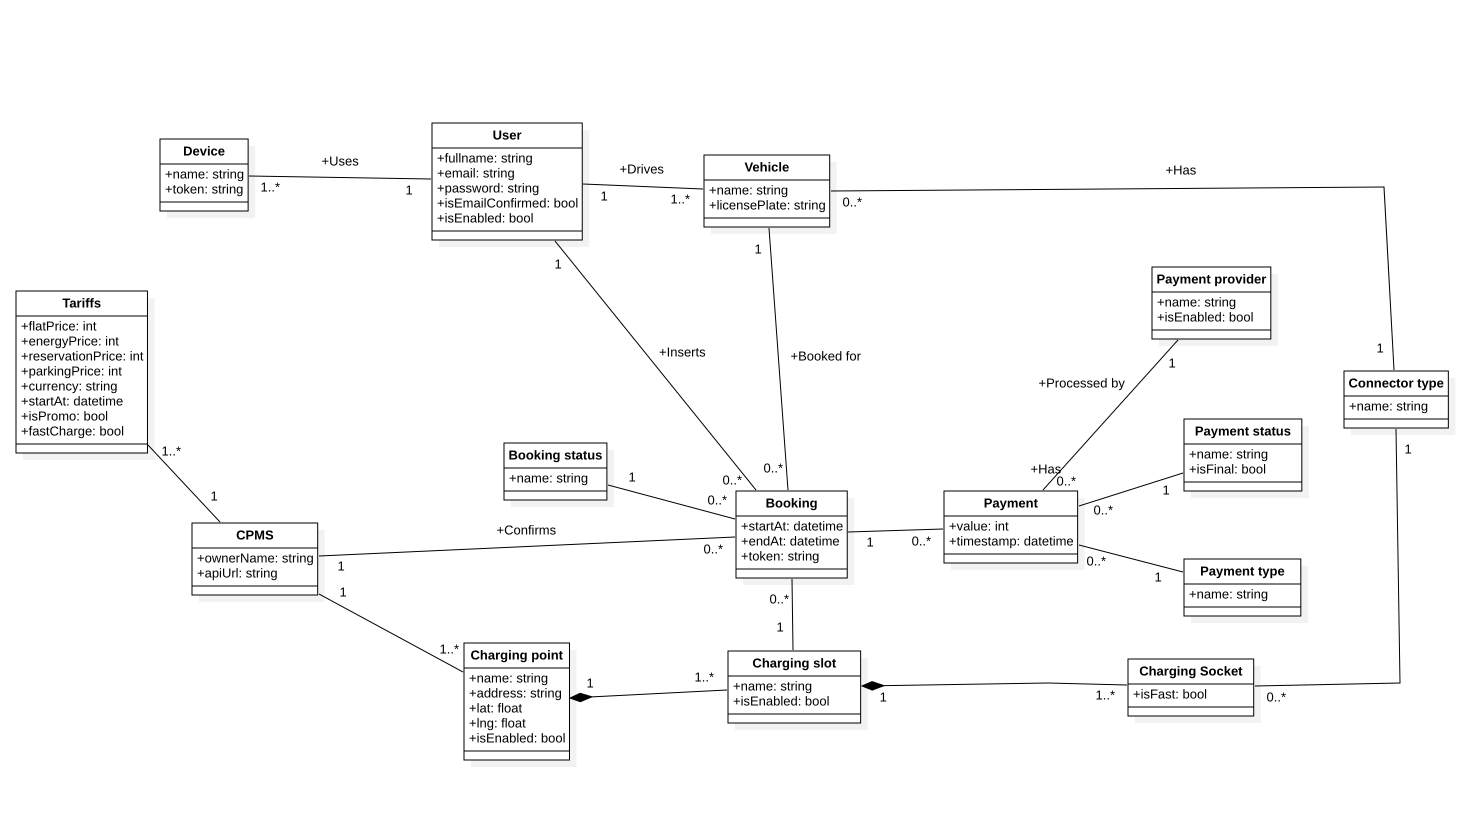
\includegraphics[width=\textwidth]{class_diagram}
\caption{Class diagram for the main models of the System}
\end{figure}
	
\clearpage
\newpage
	
\section{Deployment view}
In this section we introduce a detailed view of the system and various component from a deployment cycle perspective. The following schemes highlight the environments and the tools to be used for the system.
	
	
\begin{figure}[h]
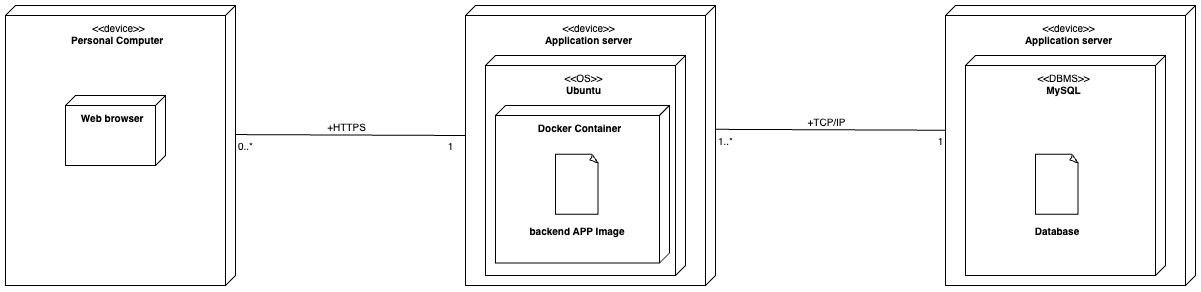
\includegraphics[width=\textwidth]{component_diagrams/deployment_diagram}
\caption{Deployment diagram for the System}
\end{figure}
	
\begin{itemize}
	\item \textbf{Personal Device}: Personal Computer used by users to run the client web application to communicate with the system
	\item \textbf{Backend Server / Virtual Private Server}: Physical device where is installed the Docker Image of the Backend APP. Multiple replicas are possibile and preferable as they will increase both reliability and availability of the system.
	\item \textbf{Database Server}: Host the database of the system. Multiple local replicas can improve read performances but also increase complexity.
\end{itemize}
	
\clearpage
\newpage
	
\section{Runtime view}
In this section are shown the sequence diagrams for the various functionalities of the system. To simplify the description there is an initial generic sequence the summarize the routing and authorization part of the request handling. Also, as all the request go through the router, the actors that sends the request to the router are omitted.
	
\subsection{Generic Routing and Authorization}
\begin{figure}[h]
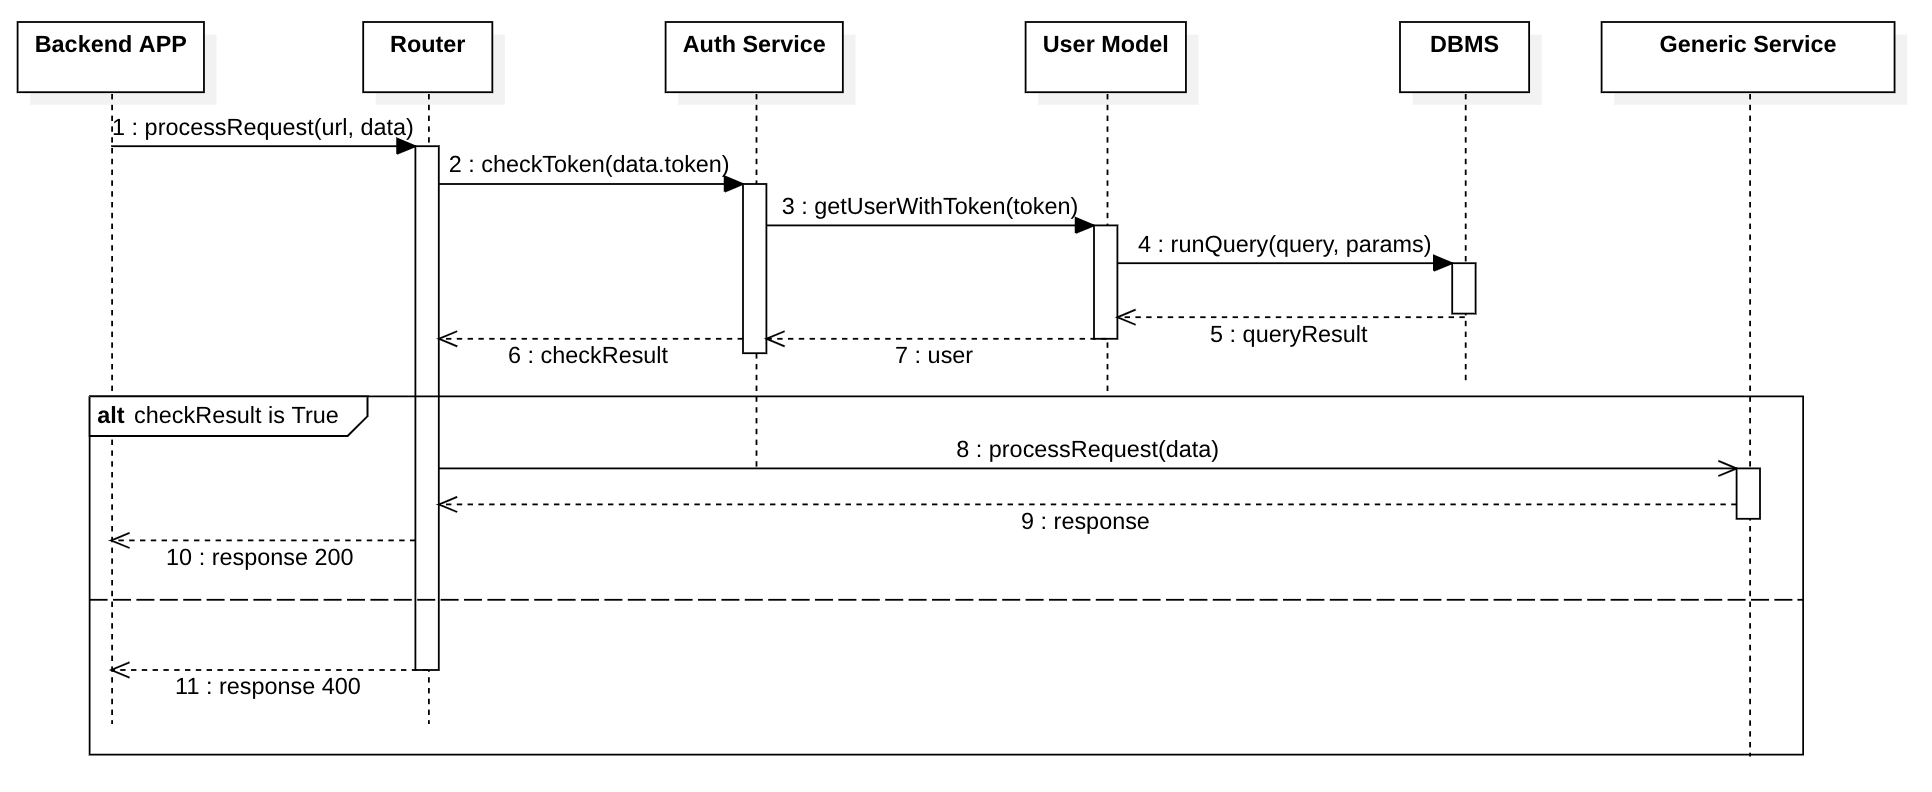
\includegraphics[width=\textwidth]{sequences/auth_request}
\caption{Generic Routing and Authorization flow for a generic request}
\end{figure}
	
When a request is received by the application web server, it goes through the Router component. It acts as an authorization middleware. 
As Authorization is needed, the whole Auth Service, Model and DBMS components are envolved.
At the end, if authorization has been completed successfully, the request is forward to the dedicated service.
	
	
\subsection{Start charging session}
\begin{figure}[h]
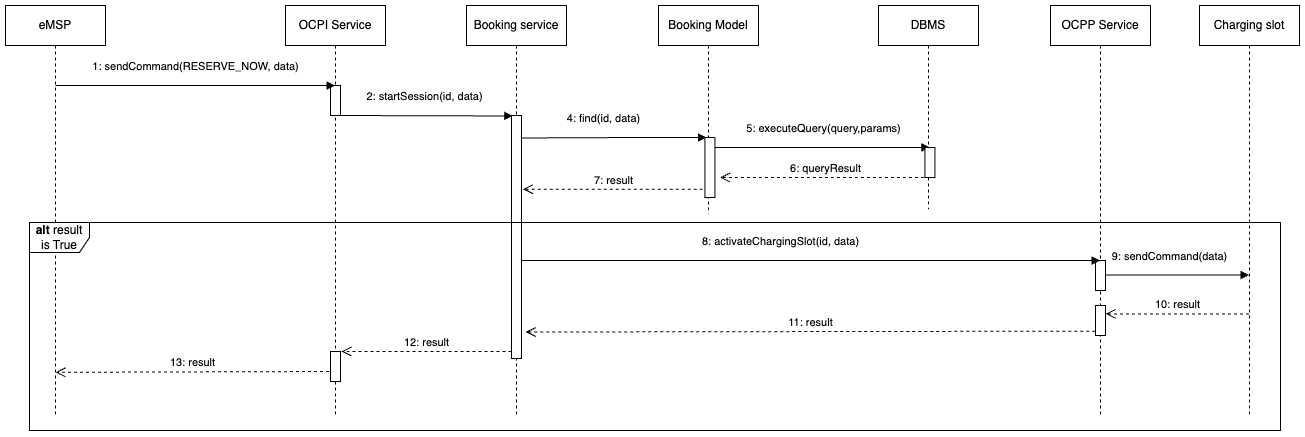
\includegraphics[width=\textwidth]{sequences/starting_session}
\caption{Start charging session}
\end{figure}
\clearpage
	
\subsection{Book a charging session}
\begin{figure}[h]
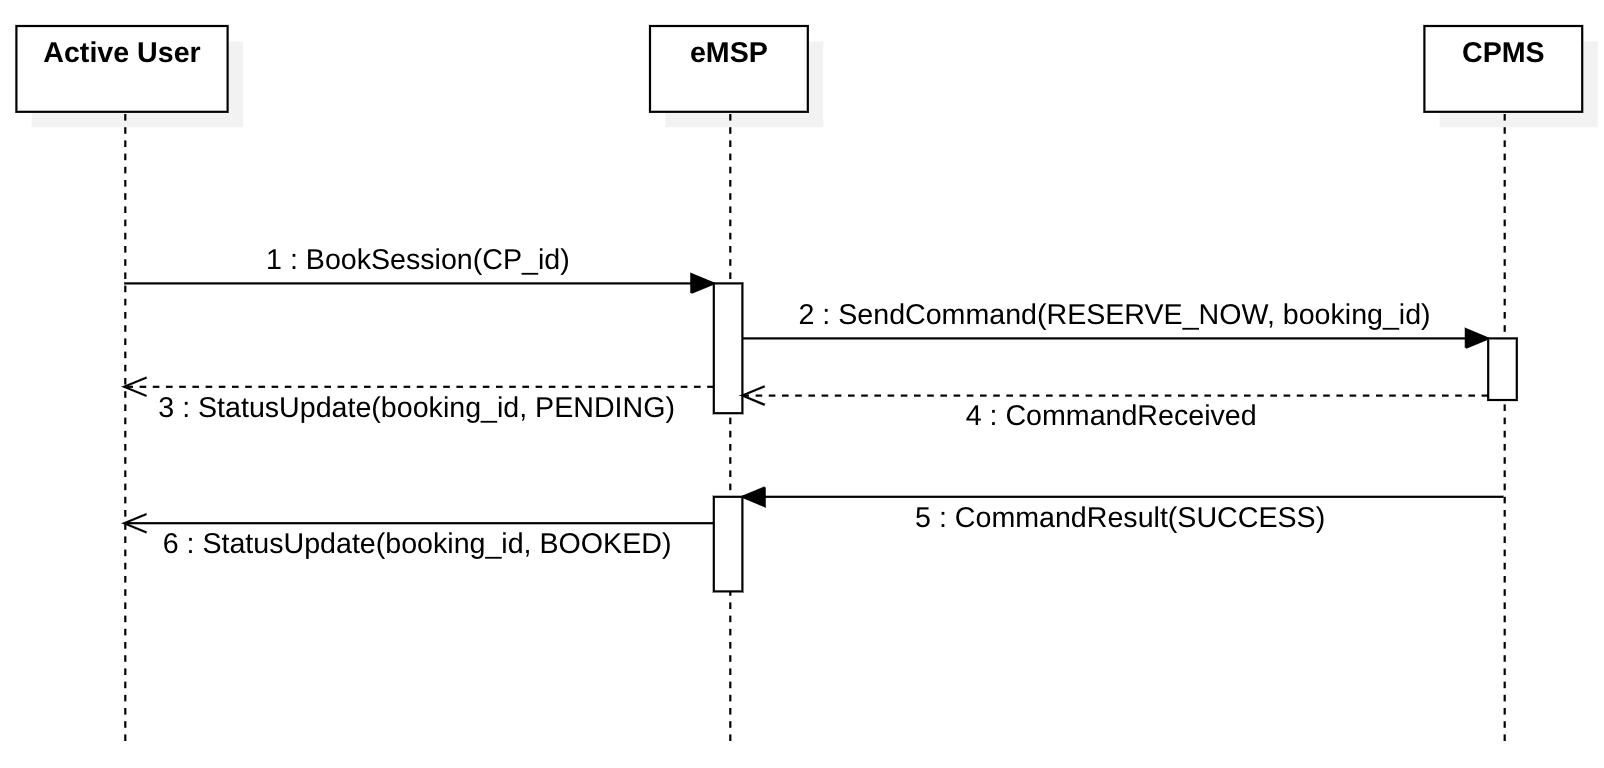
\includegraphics[width=\textwidth]{sequences/book_session}
\caption{Book a charging session}
\end{figure}

	
\section{Selected architectural style and patterns}
\begin{itemize}
	\item \textbf{Three-tier architecture}: As stated before the three-tier architecture was chosen because our system is not the producer of the data, and that there is the need for implementing different functionalities (e.g. payments) and external services.
	\item \textbf{Monolith architecture}: To simplify the development and the deployment of the system, to avoid the so called "vendor lock-in" by choosing a specific service provider for the microservices infrastructure and mainly because no usage spikes are expected, the monolith architecture has been chosen. That means that all the application server replicas contains the whole backend application and not the single services.
	\item \textbf{Authentication with Access Token}: As there are no specific requirements on the authentication functionality, the simply access token pattern can be considered a good suit for the system. 
\end{itemize}

















